\section{Polynomials and Distributions}
For reference we include the polynomial, distribution, and quadrature definitions for the continuous distributions used in this document.  To describe polynomials, we make use of the Pachhammer symbol $(a)_n$
\begin{equation}
(a)_n=a(a+1)(a+2)...(a+n-1),\hspace{10pt}n=1,2,3,...
\end{equation}
with $(a)_n=1$.  The generalized hypergeometric series $_rF_s$ is given by
\begin{equation}
_rF_s(a_1,...,a_r;b_1,...,b_s;z)=\sum_{k=0}^\infty \frac{(a_1)_k\cdots(a_r)_k}{(b_1)_k\cdots(b_s)_k}\frac{z^k}{k!}.
\end{equation}
\begin{figure}[h!]
\centering
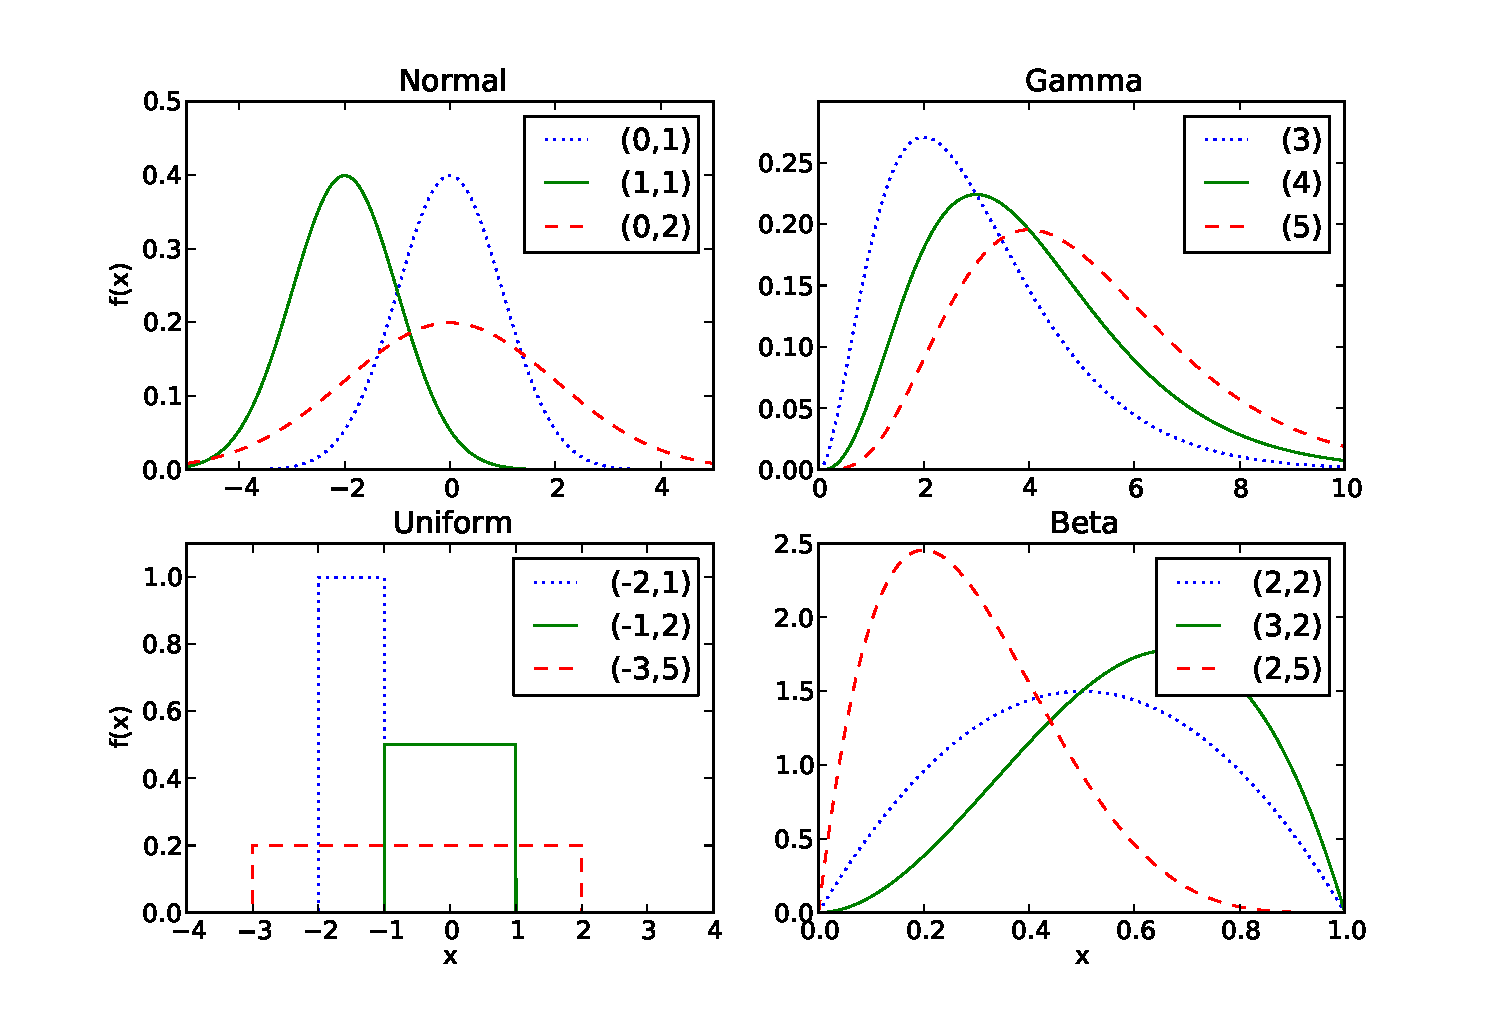
\includegraphics[width=\linewidth]{./graphics/distros}
\caption{Several Distributions}
\label{fig:distros}
\end{figure}

\subsection{Standard Distributions}
There are several standard distributions for which quadratures with corresponding polynomials are well-known, making them efficiently represented with small quadratures.  We present four here: normal, Gamma, uniform, and Beta.

\newpage
\subsubsection{Normal and Hermite $\He_n$}
The normal or Gaussian distribution has support from $-\infty$ to $\infty$ and is characterized by Hermite polynomials, with the associated Gauss-Hermite quadrature.  The pdf of the normal distribution has the form
\begin{equation}
\xi(x;\mu,\sigma^2)=\frac{1}{\sqrt{2\pi\sigma^2}}\exp\left(-\frac{(x-\mu)^2}{2\sigma^2}\right),
      \hspace{10pt} x\in(-\infty,\infty),
\end{equation}
where $\mu,\sigma^2$ are the mean and variance respectively.  Two different kinds of Hermite polynomials exist: one the ``probabilist" Hermite polynomial $\He_n(x)$, and the more often seen ``physicist'' Hermite polynomial $H_n(x)$.  The two are essentially the same with the important exception $H_n(x/\sqrt{2})=\He_n(x)$.
\begin{align}
\He_n&=(-1)^n e^{x^2/2}\frac{d^n}{dx^n}e^{-x^2/2},\\
H_n&=(-1)^n e^{x^2}\frac{d^n}{dx^n}e^{-x^2}.
\end{align}
We make use of the probabilist here because of its conformity with the Gaussian distribution.  The Hermites are orthogonal,
\begin{equation}
\intf \He_m(x)\He_n(x) e^{-x^2/2}dx=\sqrt{2\pi} n! \delta_{nm}.
\end{equation}
The weighting function is given by
\begin{equation}
W_{\He}(x)=e^{-x^2/2}.
\end{equation}
Hermite quadrature integrates exactly functions of the kind
\begin{equation}
\intf f(x)e^{-x^2/2}dx=\sum_{\ell=0}^L w_\ell f(x_\ell).
\end{equation}
The abscissas of the quadrature are given by roots of the $\He_n$ polynomial and weights are given by
\begin{equation}
w_\ell = \frac{L!\sqrt{2\pi}}{n^2[\He_{n-1}(x_\ell)]^2}.
\end{equation}
A normal distribution is shown with $\mu=0,\sigma^2=1$ in Fig. \ref{fig:distros}.

\newpage
\subsubsection{Gamma and Laguerre $L_n^\alpha$}
The Gamma distribution has support from 0 to $\infty$ and is characterized by Laguerre polynomials with the associated Gauss-Laguerre quadrature.  The pdf of the Gamma distribution has the form
\begin{equation}
\xi(x;\alpha,\beta)=\frac{x^\alpha e^{-x/\beta}}{\beta^{\alpha+1}\Gamma(\alpha+1)},
    \hspace{10pt}\alpha>-1,\beta>0,x\in(0,\infty),
\end{equation}
\begin{equation}
\Gamma(\alpha)\equiv\int_0^\infty t^\alpha e^{-t}\frac{dt}{t},
\end{equation}
\begin{equation}
\Gamma(\alpha+1)=\alpha\Gamma(\alpha),
\end{equation}
where $\alpha,\beta$ are shape and scale constants, respectively.  The (generalized) Laguerre polynomials $L^{(\alpha)}_n$ are the solutions to the second order PDE
\begin{equation}
xy''+(\alpha+1-x)y'+ny=0,
\end{equation}
and are given by
\begin{align}
L^{(\alpha)}_n(x)&=\frac{x^{-\alpha}e^x}{n!}\frac{d^n}{dx^n}\left(e^{-x}x^{n+\alpha}\right),\\
  &=\frac{(\alpha+1)_n}{n!} {}_1F_1(-n;\alpha+1;x),
\end{align}
\begin{equation}
\int_0^\infty e^{-x} x^\alpha L^{(\alpha)}_m(x) L^{(\alpha)}_n(x)dx=\frac{\Gamma(n+\alpha+1)}{n!}\delta_{mn},
     \hspace{10pt}\alpha>-1.
\end{equation}
The weighting function is given by
\begin{equation}
W_{L^{(\alpha)}}(x)=e^{-x}x^\alpha.
\end{equation}
General Laguerre quadrature exactly integrates functions of the kind
\begin{equation}
\int_0^\infty  f(x)e^{-x} x^\alpha dx=\sum_{\ell=0}^N w^{(\alpha)}_\ell f(x^{(\alpha)}_\ell).
\end{equation}
The abscissas of the quadrature are the roots of the polynomial $L^{(\alpha)}_n$, and the weights are given by
\begin{equation}
w^{(\alpha)}_\ell=\frac{1}{x^{(\alpha)}_\ell}\left(\drv{}{x}L_N^{(\alpha)}(x^{(\alpha)}_\ell)\right)^{-1}.
\end{equation}
A Gamma distribution with shape $\alpha=3$ and scale $\beta=1$ is shown in Fig. \ref{fig:distros}.

\newpage
\subsubsection{Uniform and Legendre $P_n$}
The uniform distribution has support from $a$ to $b$, but is typically defined over the domain [-1,1], and is characterized by Legendre polynomials with the associated Gauss-Legendre quadrature.  The pdf of the uniform distribution is flat between $a$ and $b$ and zero everywhere else,
\begin{equation}
\xi(x;a,b)=\frac{1}{b-a},\hspace{20pt}x\in[a,b],
\end{equation}
where $a,b$ are the maximum and minimum value, respectively.  The Legendre polynomials $P_n(x)$ are solutions to the PDF
\begin{equation}
\drv{}{x}\left[(1-x^2)\drv{}{x}P_n(x)\right]+n(n+1)P_n(x)=0,
\end{equation}
and are given by
\begin{equation}
P_n(x)=\frac{1}{2^nn!}\frac{d^n}{dx^n}\big[(x^2-1)^2\big],
\end{equation}
\begin{equation}
\int_{-1}^{1} P_m(x)P_n(x)dx=\frac{2}{2n+1}\delta_{mn}.
\end{equation}
It should be noted that shifting $P_n(x),x\in[-1,1]$ to $P_n(z),z\in[a,b]$ is performed by the transformation
\begin{equation}
P_n(z)=\frac{b-a}{2}P_n\left(\frac{b-a}{2}x+\frac{a+b}{2}\right),\hspace{10pt}x\in[-1,1],z\in[a,b].
\end{equation}
The weighting function is given by
\begin{equation}
W_{P}(x)=1.
\end{equation}
Legendre quadrature exactly integrates functions of the kind
\begin{equation}
\into f(x)dx=\sum_{\ell=0}^L w_\ell f(x_\ell).
\end{equation}
The abscissas of the quadrature are the roots of the polynomial $P_n$, and the weights are given by
\begin{equation}
w_\ell=\frac{2}{(1-x_\ell^2)\left[\drv{}{x}P_n(x_\ell)\right]^2}.
\end{equation}
A uniform distribution with minimum -1 and double-range 2 is shown in Fig. \ref{fig:distros}.

\newpage
\subsubsection{Beta and Jacobi $P_n^{(\alpha,\beta)}$}
The Beta distribution has the same support as the uniform distribution, $a$ to $b$, but is often defined over the domain [0,1], and is characterized by Jacobi polynomials with associated Jacobi quadrature.  The Legendre polynomials are a particular type of the Jacobi polynomials with $\alpha=\beta=0$.  The pdf of the beta distribution is given by
\begin{equation}
\xi(x;\alpha,\beta)=\frac{x^{\alpha-1}(1-x)^{\beta-1}}{B(\alpha,\beta)}, \hspace{10pt} x\in[0,1],
\end{equation}
\begin{equation}
B(\alpha,\beta)=\int_0^1 t^{\alpha-1}(1-t)^{\beta-1} dt,
\end{equation}
where $\alpha,\beta$ are shape parameters.  The Jacobi polynomials are given by
\begin{align}
P_n^{(\alpha,\beta)}(x)&=\frac{(-1)^n}{2^nn!}(1-x)^{-\alpha}(1+x)^{-\beta}\frac{d^n}{dx^n}
  \left[(1-x)^-\alpha(1+x)^\beta(1-x^2)^n \right],\\
  &=\frac{(\alpha+1)_n}{n!}{}_2F_1\left(-n,1+\alpha+\beta+n;\alpha+1;\frac{1-x}{2}\right),
\end{align}
\begin{equation}
\into(1-x)^\alpha(1+x)^\beta P_m^{(\alpha,\beta)}(x)P_n^{(\alpha,\beta)}(x)dx=
    \frac{2^{\alpha+\beta+1}}{2n+\alpha+\beta+1}
    \frac{\Gamma(n+\alpha+1)\Gamma(n+\beta+1)}{\Gamma(n+\alpha+\beta+1)n!}\delta_{mn}.
\end{equation}
The weighting function is given by
\begin{equation}
W_{P^{(\alpha,\beta)}}(x)=(1-x)^\alpha (1+x)^\beta.
\end{equation}
Jacobi quadrature exactly integrates functions of the kind
\begin{equation}
\into f(x) (1-x)^\alpha(1+x)^\beta dx = \sum_{\ell=0}^L w_\ell f(x_\ell).
\end{equation}
The abscissas of the quadrature are the roots of the polynomial $P_n^{(\alpha,\beta)}$, and the weights are given by
\begin{equation}
w_\ell=-\frac{(2n+\alpha+\beta+2)}{(n+\alpha+\beta+1)}
  \frac{\Gamma(n+\alpha+1)\Gamma(n+\beta+1)}{\Gamma(n+\alpha+\beta+1)(n+1)!}
  \frac{2^{\alpha+\beta}}{P_{n+1}(x_\ell)\drv{}{x}P_n(x_\ell)}.
\end{equation}
A beta distribution with $\alpha=2,\beta=2$ is shown in Fig. \ref{fig:distros}.

\newpage

\subsection{Non-Standard Distributions}
There are many other distributions commonly used in uncertainty, but without a convenient set of polynomials and quadrature to fit them.  Because of the widespread use of these distributions, we present some here with approaches to representation by quadrature and polynomials.
\begin{figure}[h!]
\centering
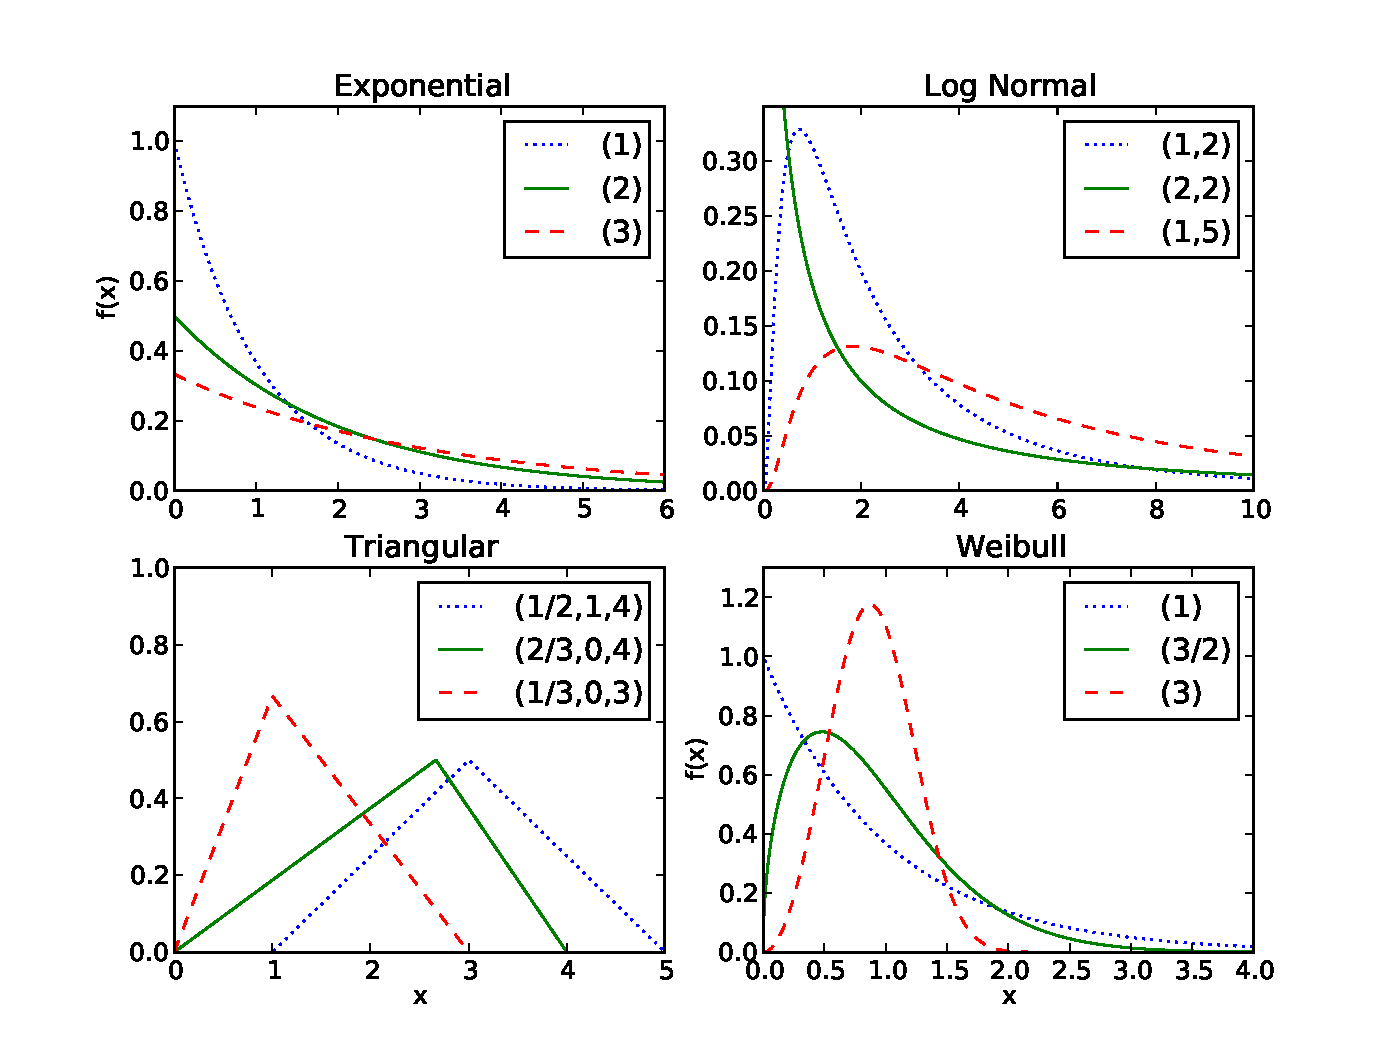
\includegraphics[width=\linewidth]{./graphics/distros_alt}
\caption{Alternate Distributions}
\label{fig:distros_alt}
\end{figure}
\subsection{Exponential}
The exponential distribution ranges from 0 to $\infty$ and has the form
\begin{equation}
\xi(x;\alpha=\alpha e^{-\alpha x}, x\in [0,\infty),
\end{equation}
where $\alpha$ is a rate scaling factor. TODO finish.

\subsubsection{Lognormal}
The log normal is descriptively the log of the normal distribution.  It ranges from 0 to $\infty$ and has the form
\begin{equation}
\xi(x;\mu,\sigma^2)=\frac{1}{x\sqrt{2\pi\sigma^2}}\exp\left(-\frac{(\ln x-\mu)^2}{2\sigma^2}\right),
  \hspace{10pt} x\in(0,\infty).
\end{equation}
where $\mu,\sigma^2$ are the mean and variance, respectively.  TODO finish.

\subsubsection{Triangular}
The triangular distribution ranges from $a$ to $b$ and rises linearly from $a$ to a point, after which it falls linearly to $b$.  The pdf is given by
\begin{equation}
\xi(x;a,b,c)=\begin{cases}
0, & x<a,\\
\frac{2(x-a)}{(b-a)(c-a)}, & a\leq x \leq c,\\
\frac{2(b-x)}{(b-a)(b-c)}, & c<x\leq b,\\
0, & b<x,
\end{cases}
\end{equation}
where $a,b,c$ are the minimum, maximum, and location of the highest point, respectively. TODO finish.

\subsubsection{Weibull}
The Weibull distribution ranges from 0 to $\infty$ and has the form
\begin{equation}
\xi(x;\lambda,k)=\frac{k}{\lambda}\left(\frac{x}{\lambda}\right)^{k-1}e^{-(x/\lambda)^k},
\end{equation}
where $\lambda,k$ are the scale and shape parameters, respectively.  Often, $\lambda=1$ and $k$ is the only shaping parameter. TODO finish.

\subsubsection{Truncated Gaussian}
The truncated Gaussian distribution ranges from $a$ to $b$ and appears as a Gaussian normal distribution truncated at $a$ and $b$ with mean $\mu$ and varianve $\sigma^2$:
\begin{equation}
\xi(x;\mu,\sigma,a,b)=\frac{\frac{1}{\sigma}g(\frac{x-\mu}{\sigma})}{G(\frac{b-\mu}{\sigma})-G(\frac{a-\mu}{\sigma})},
    \hspace{10pt} x\in[a,b],
\end{equation}
where $g$ is the pdf of a normal distribution with $\mu=0,\sigma^2=1$ and $G$ is its cdf.  This can be rewritten as
\begin{equation}
\xi(x;\mu,\sigma,a,b)=\frac{1}{2\sqrt{s\pi\sigma^2}}\left(
\frac{\exp\left(-\frac{(x-\mu)^2}{2\sigma^2}\right)}{\erf(\frac{b-\mu}{\sigma\sqrt{2}})-\erf(\frac{a-\mu}{\sigma\sqrt{2}})}
\right),\hspace{10pt} x\in[a,b],
\end{equation}
where erf is the error function.

\subsubsection{Arbitrary}
Many other distributions may arise in characterizing the uncertainty of input parameters.  In the event none of the above distributions are close enough, using the distribution's ppf to represent it using shifted Legendre polynomials is recommended, with care for the number of terms used.